

\subsection{Matriz PEYEA}
Esta matriz permite definir si una estrategia activa, conservadora, defensiva o competitiva es la más adecuada para una organización dada. Los ejes de la matriz representan dos dimensiones internas (fuerza financiera y ventaja competitiva) y dos externas (fuerza de la industria y estabilidad del ambiente). Se seleccionan variables para cada una de las dimensiones; se les adjudica una calificación con un valor numérico de 1 a 6, o –1 a –6, donde 1 representa la mejor calificación en valor absoluto; se calcula la calificación promedio de cada dimensión; se anotan las calificaciones promedio de cada dimensión en el eje correspondiente; se suman las dos calificaciones del eje X para obtener una primera coordenada, y se repite para el eje de las Y; por último, se traza un vector del origen al punto encontrado para ubicar en un cuadrante el perfil que la empresa debiera buscar para orientar su estrategia.\cite{DOFA}

la definicion del acronimo PEYEA es la siguiente:
\begin{itemize}
    \item \textbf{P - Posición Estratégica:} Es la situación actual de la empresa en el mercado.
    \item \textbf{E - Evaluación:} Es el análisis de la posición estratégica actual.
    \item \textbf{Y - Yuxtaposición:} Es la comparacion de la posición estratégica con las condiciones del mercado y la competencia.
    \item \textbf{E - Estrategia:} Teniendo en cuenta la evaluación y analisis se plantea una estrategia.
    \item \textbf{A - Acción:} Son las acciones que se deben realizar para llevara cabo la estrategia planteada.
\end{itemize}

\subsection{Pasos para elaborar una matriz PEYEA}

\begin{enumerate}
    \item \textbf{Seleccionar Variables:} Elegir una serie de variables que representen las cuatro dimensiones de la matriz (Fuerzas Financieras, Ventaja Competitiva, Estabilidad del Ambiente y Fuerza de la Industria). Resaltando la importancia de estas variables para la organización y el mercado.
    \item \textbf{Asignar Valores Numéricos:} Asignar un valor numérico a cada variable. Para las Fuerzas Financieras(FF) y Fuerza de la Industria(FI), utilizar una escala de +1 (peor) a +6 (mejor). Para Ventaja Competitiva(VC) y Estabilidad del Ambiente(EA), utilizar una escala de -1 (mejor) a -6 (peor).
    \item \textbf{Calcular la Calificación Promedio:} se suman los valores resultantes de las variables de cada dimensión y se divide el total por la cantidad de variables para obtener la media.
    \item \textbf{Anotar en la Matriz:} Ubicar los valores resultados en el calculo anterior de cada factor en el eje correspondiente de la matriz.
    \item \textbf{Sumar los Valores de los Ejes:} Sumar los valores medios de las Fuerzas Financieras y Ventaja Competitiva para el eje vertical, y Estabilidad del Ambiente y Fuerza de la Industria para el eje horizontal.
    \item \textbf{Determinar la Posición Estratégica:} Dependiendo de la intersección de los valores en la matriz se adopatará la estrategia recomendable ya sea agresiva, conservadora, defensiva o competitiva.
    \item \textbf{Trazar un Vector Direccional:} Desde el origen de la matriz hasta el punto de intersección,se debe trazar un vector.Dando guia del tipo de estrategia más adecuada para la organización.
\end{enumerate}

Comprendiendo los conceptos y pasos descritos anteriormente, se procede a elaborar la matriz PEYEA para la empresa en cuestión. Esta matriz permitirá identificar las estrategias más adecuadas para mejorar el desempeño de la compañía en el mercado y determinar si estas son agresivas, conservadoras, defensivas o competitivas.

\vspace{2mm}
\begin{minipage}{0.9\textwidth}
\centering
\captionof{table}[{Matriz PEYEA.}]{ Matriz PEYEA }
\label{peyea}
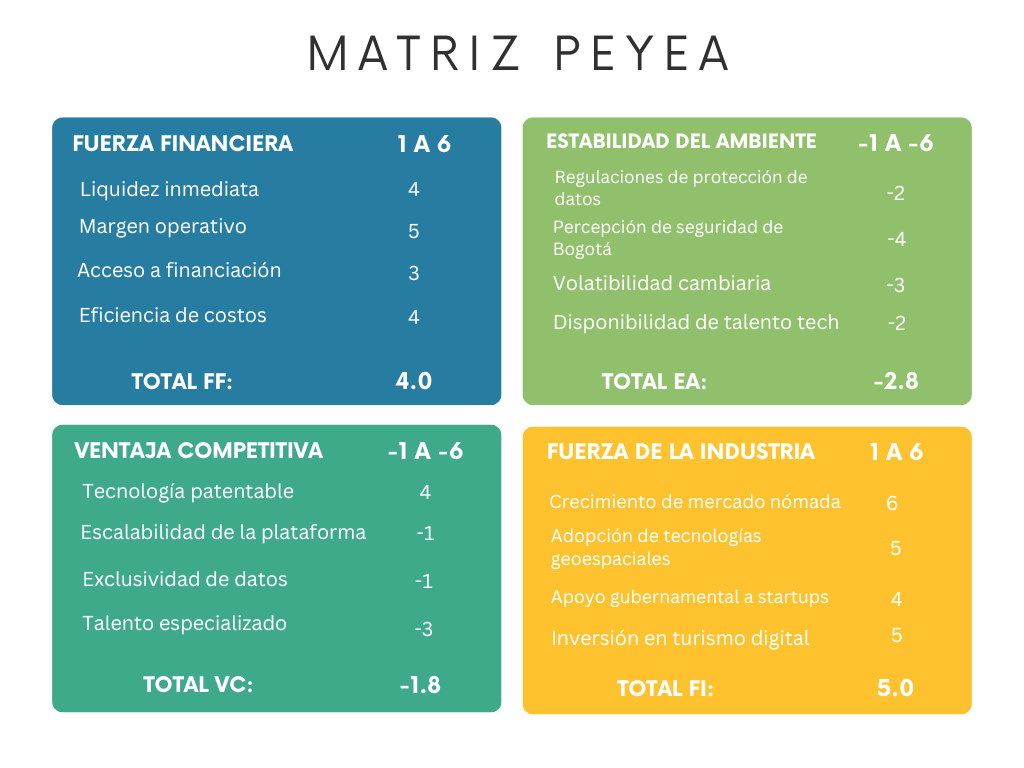
\includegraphics[scale=0.5]{Content/Images/Matriz PEYEA.png}
%\fnote{Nota. \textup{Fuente : Autores.}}
\end{minipage}

Para determinar el valor de X, se sumaron los valores de Ventaja Competitiva (VC) y Fuerza de la Industria (FI).Como se muestra a continuación:
\begin{align*}
X &= VC + FI \\
X &= -1.8+5 \\
X &= 3.2
\end{align*}

El valor de Y se obtuvo sumando Fuerza Financiera (FF) y Estabilidad del Ambiente (EA).Como se muestra a continuación:
\begin{align*}
Y &= FF + EA \\
Y &= 4.0-2.8 \\
Y &= 1.2
\end{align*}

Dichos valores se representan gráficamente en la siguiente imagen:

\vspace{2mm}
\begin{minipage}{0.9\textwidth}
\centering
\captionof{figure}[{Representación gráfica Matriz PEYEA.}]{ Representación gráfica Matriz PEYEA }
\label{peyeagrafico}
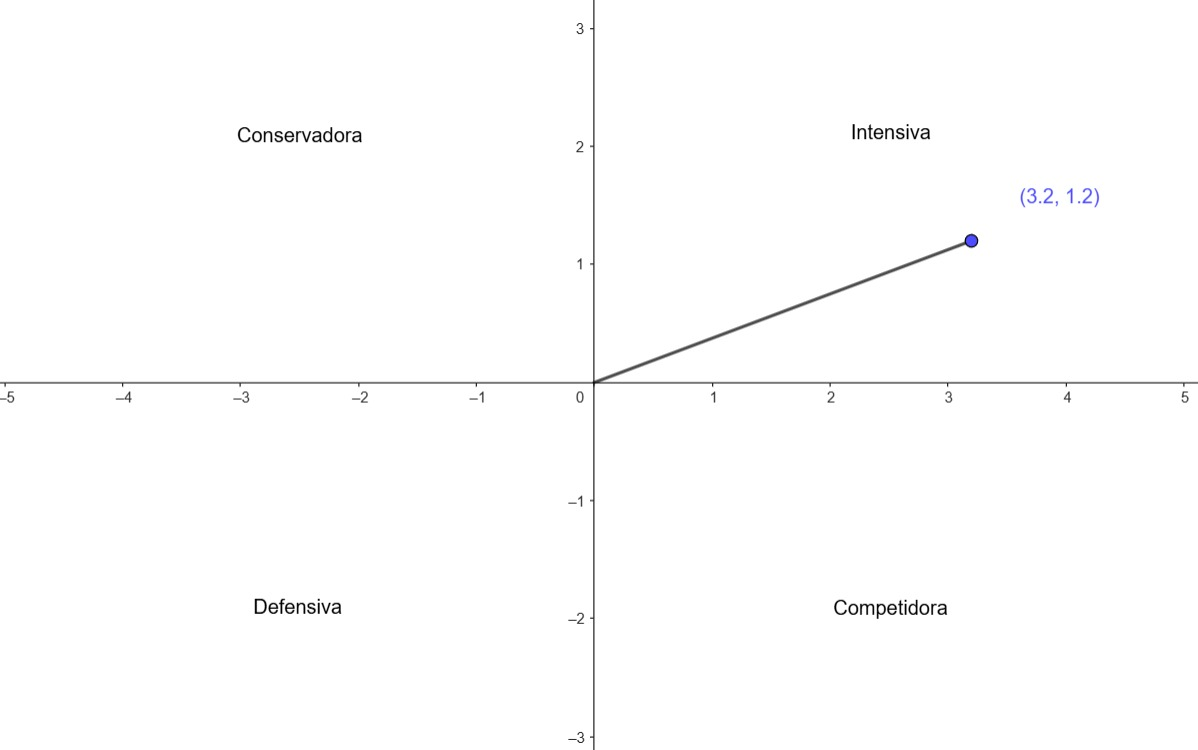
\includegraphics[width=1\textwidth]{Content/Images/PEYEA.jpeg}
%\fnote{Nota. \textup{Fuente : Autores.}}
\end{minipage}

Como conclusión, se obtiene que el proyecto se encuentra en el primer cuadrante de la matriz PEYEA, indicando que se debe seguir una estrategia intensiva. Indicando que las fortalezas internas son un pilar importante para maximizar las oportunidades externas, explotando las ventajas competitivas y la fuerza financiera del proyecto. Permitiendo maxificar las fortalezas y oportunidades, minimizando las debilidades y amenazas,garantizando así un crecimiento sostenido y una posición competitiva sólida en el mercado para el proyecto.
%------------------------------------------------------------------